\section*{Problema 5}

\textbf{En este ejercicio usamos resultados del heptatlón feminina de los pasados juegos olímpicos de Tokyo (2021). En el archivo heptatlonTokyose pueden consultar los tiempos/distancias y el puntaje final (score) de 20 atletas.}

\textbf{a) Describe de manera general los datos sin considerar la columna con los puntajes finales, usando visualizaciones ilustrativas. Toma en cuenta que son pocas observaciones. Asi, no será posible llegar a conclusiones fuertes.}

Los datos obtenidos de los resultados del heptatlón femenino de los juegos olímpicos del 2021 contienen la siguiente información:

\begin{enumerate}
    \item \textbf{Salto de altura (high jump)}
    \item \textbf{Lanzamiento de peso (shot put)}
    \item \textbf{Salto de longitud (long jump)}
    \item \textbf{Lanzamiento de javalina (javelin)}
    \item \textbf{100 metros planos (100m)}
    \item \textbf{200 metros planos (200m)}
    \item \textbf{800 metros planos (800m)}
\end{enumerate}

Las competencias de los puntos 1 al 4 el objetivo es obtener la mayor distancia posible. En cambio las competencias de los puntos 5 al 8 el objetivo es obtener el menor tiempo posible.

Las distancias y tiempos obtenidos por los atletas fueron normalizadas con la ecuación \ref{eq:normalization}.

\begin{equation}
    m_n = \frac{m - \mu}{\sigma} \label{eq:normalization}
\end{equation}

donde

\begin{itemize}
    \item $m$ es la distancia o tiempo obtenido en la prueba del atleta.
    \item $\mu$ es la media de los atletas en cierta prueba.
    \item $\sigma$ es la desviación estandar de los atletas en cierta prueba.
    \item $m_n$ es la medida de la distancia o tiempo del participante estandarizado.
\end{itemize}

En la figura \ref{fig:estandar_points} se visualizan las medidas $m_n$ de cada prueba. En la parte superior se encuentran las pruebas donde es mejor obtener un puntaje alto y en la parte inferior las pruebas donde es mejor obtener un puntaje bajo.

\begin{figure}[H]
    \centering
    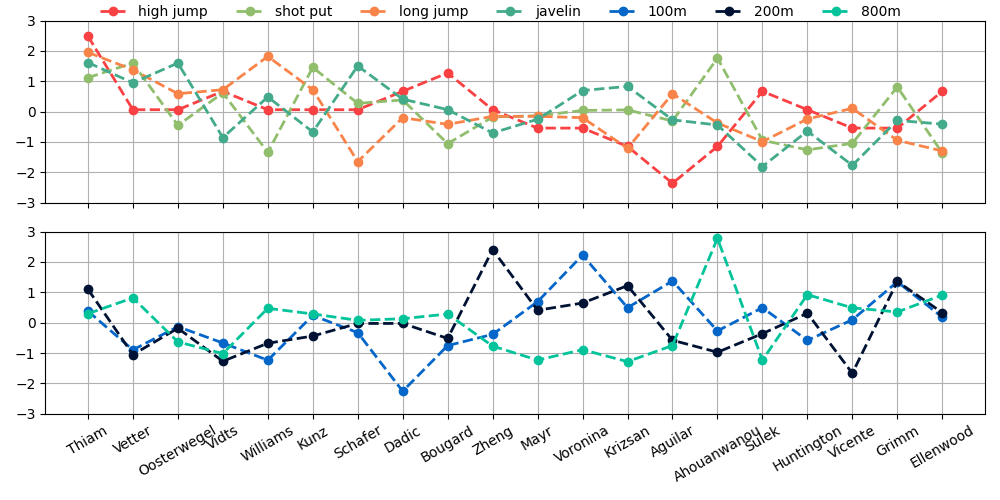
\includegraphics[width=16cm]{Graphics/heptatlon.png}
    \caption{Puntajes estandarizados de los atletas obtenidos en los olímpicos 2021.}
    \label{fig:estandar_points}
\end{figure}

Con la figura \ref{fig:estandar_points} se puede visualizar que atleta es mejor en que prueba y el rendimiento general de cada uno.

\textbf{b) Un problema en un heptatlón es cómo convertir los resultados obtenidos en las diferentes pruebas en un puntaje final. Explora la utilidad de PCA usando la proyección de los resultados de las pruebas sobre el primer componente como una alternativa al puntaje final. ¿Cómo se relaciona con el puntaje final oficial? Información sobre cómo se calcula actualmente el puntaje: \href{http://theaftermatter.blogspot.mx/2012/06/maths-of-heptathlon-why-scoring-system.html}{Puntaje heptatlon}.}

\begin{figure}[H]
    \centering
    \includegraphics[width=10cm]{Graphics/heptatlon_pca.png}
\end{figure}